\section{RQ2: Which pipeline decisions matter}
\label{sec:ladder}

\subsection{Cumulative ablation on COCO val2017}

\Cref{fig:timeline} illustrates the three schedules. \Cref{tab:ladder}
and \cref{fig:ladder} report the cumulative ladder on
all 5,000 val2017 images. Model, engine and accuracy are fixed.

\begin{figure*}[t]
\centering
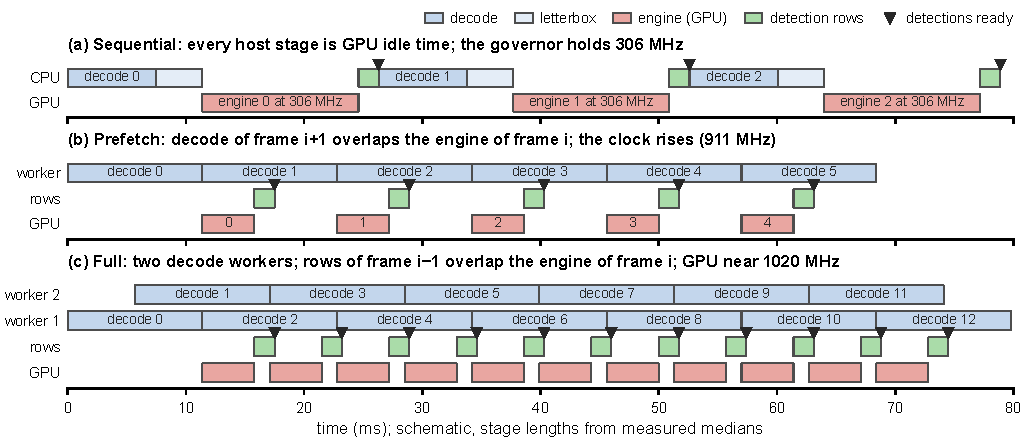
\includegraphics[width=\textwidth]{figs/timeline.pdf}
\caption{Schematic of the three schedules. The time axis uses the measured stage medians of the sequential
float pipeline of \cref{sec:diagnosis}: decode 7.5\,ms, letterbox
3.9\,ms, rows ${\approx}1.5$\,ms and engine 13.2\,ms (host-measured
enqueue-to-completion at 306\,MHz; the device-side CUDA-event share is
12.5\,ms, \cref{tab:fixedfreq}). The stage medians sum to 26.0\,ms,
while the measured period is 29.5\,ms (33.9 images/s). The difference
is per-image main-thread work outside the timed stages.
Markers ($\blacktriangledown$) show
when each frame's detections become ready. The bars show the structure,
not the measured throughputs. In (a) every host stage is GPU
idle time, so the governor holds the minimum clock. In (b) and (c) the
host stages overlap engine execution.}
\label{fig:timeline}
\end{figure*}

\begin{table*}[t]
\centering
\caption{Cumulative pipeline ablation for YOLO26n at 640 on all 5,000 COCO val2017
images (batch 1, FP16 TensorRT, \texttt{MAXN\_SUPER}). Each cell is the mean of three
rotated runs; run-to-run throughput ranges are below 2.5\% of the mean for every
cell except the float sequential pipeline under default governors (33.1--34.3 images/s) and prefetch with stream synchronization under default governors (111.5--119.1 images/s). The $\dagger$ row is a diagnostic, not a cumulative step: it reverts the previous rung's event synchronization to isolate its effect (\cref{sec:sched}). The last two rows are variants of the full uint8 pipeline.
AP is official COCOeval. Each row's predictions were byte-identical across
all six runs (both clock settings), and rows with the same input type share one
prediction file, except the Ultralytics baseline, which exports its own
engine and has its own prediction hash. GPU MHz is the mean sampled \texttt{devfreq} clock under the default
governor (always 1020 when locked). CPU ms is process CPU time per
image; W is mean module input power (\texttt{VDD\_IN} rail). Table headers
abbreviate images per second as img/s.}
\label{tab:ladder}
\small
\setlength{\tabcolsep}{3.4pt}
\begin{tabular}{lcc rrrrr rrr}
\toprule
& & & \multicolumn{5}{c}{Default governors} & \multicolumn{3}{c}{\texttt{jetson\_clocks}} \\
\cmidrule(lr){4-8} \cmidrule(lr){9-11}
Pipeline & AP & AP$_S$ & img/s & mJ/img & W & GPU MHz & CPU ms & img/s & mJ/img & W \\
\midrule
Ultralytics \texttt{predict} & 0.4026 & 0.1978 & 31.1 & 194.6 & 6.06 & 306 & 20.5 & 73.9 & 139.3 & 10.29 \\ \midrule
Ours: float input, sequential & 0.4024 & 0.1975 & 33.9 & 187.6 & 6.36 & 306 & 21.9 & 59.9 & 165.3 & 9.90 \\
+ in-graph uint8 preprocessing & 0.4026 & 0.1977 & 40.1 & 156.1 & 6.26 & 306 & 17.8 & 90.1 & 119.1 & 10.74 \\
+ event synchronization & 0.4026 & 0.1977 & 50.0 & 150.7 & 7.54 & 306 & 21.5 & 90.4 & 119.9 & 10.84 \\
$\dagger$ + decode prefetch (stream sync) & 0.4026 & 0.1977 & 116.1 & 83.7 & 9.72 & 736 & 13.5 & 158.6 & 86.2 & 13.67 \\
+ decode prefetch & 0.4026 & 0.1977 & 146.6 & 87.2 & 12.77 & 911 & 12.7 & 159.4 & 87.2 & 13.90 \\
+ post-processing overlap & 0.4026 & 0.1977 & 175.2 & 81.2 & 14.23 & 999 & 10.6 & 182.6 & 80.5 & 14.69 \\
+ second decode worker & 0.4026 & 0.1977 & 213.8 & 74.5 & 15.94 & 1019 & 11.6 & 217.9 & 74.5 & 16.24 \\ \midrule
Full scheduling, float input & 0.4024 & 0.1975 & 89.2 & 109.9 & 9.80 & 599 & 21.6 & 98.5 & 122.2 & 12.03 \\ \midrule
Full, arrival-aware overlap & 0.4026 & 0.1977 & 194.8 & 77.9 & 15.17 & 1011 & 12.8 & 214.2 & 75.2 & 16.12 \\
Full, GC paused in timed loop & 0.4026 & 0.1977 & 230.2 & 71.6 & 16.49 & 1016 & 11.2 & 231.8 & 72.4 & 16.79 \\
\bottomrule
\end{tabular}
\end{table*}


\begin{figure*}[t]
\centering
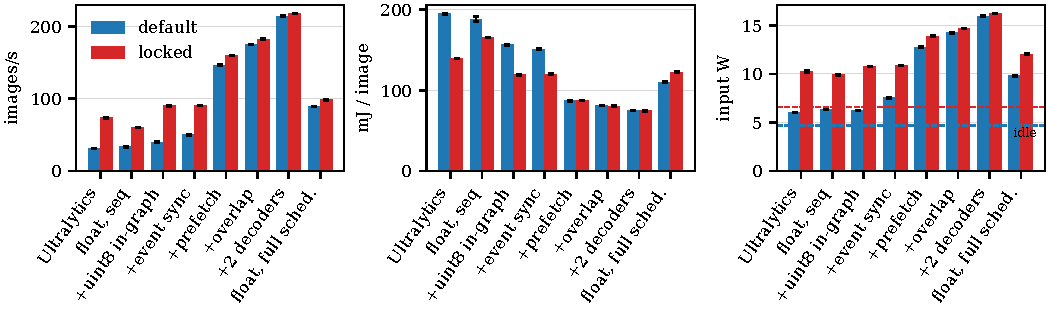
\includegraphics[width=\textwidth]{figs/ladder.pdf}
\caption{Throughput, energy per image and mean input power along the
ladder of \cref{tab:ladder} (bars: mean; whiskers: minimum--maximum of
three runs). Dotted lines in (c) mark idle input power
(4.68\,W default, 6.62\,W locked).}
\label{fig:ladder}
\end{figure*}

\textbf{Accuracy.}
The uint8 pipeline scores 0.40257 AP and 0.19766 AP$_S$, against 0.40259
and 0.19779 for the Ultralytics predictor on its own engine; the
float-input variant scores 0.40240. The ${\approx}0.6$-point gap to the
40.9 AP reported for YOLO26n on a desktop GPU with its own
export~\cite{jocher2026yolo26} is thus a property of the evaluation
stack, not of the pipeline. Agreement required one
decoder fix: an earlier version subtracted the fractional letterbox
padding instead of the integer placement offset, which shifted boxes by
half a pixel for odd padding and measurably lowered AP on the
verification split. Every pipeline was therefore checked with official
COCOeval on the full split.

\textbf{Baselines.}
Under default governors the Ultralytics predictor and the float-input
sequential pipeline reach 31.1 and 33.9 images/s, with the GPU at
306\,MHz throughout. Locking clocks with \texttt{jetson\_clocks}, the
usual benchmarking recommendation on Jetson~\cite{nvidia2024jetsonperf},
raises them to 73.9 and 59.9 images/s at 3.5--4.2\,W more input power.

\textbf{Host-side changes help a sequential schedule only through the host.}
Moving normalization and the channel transpose into the engine saves
4.1\,ms of CPU time per image and raises throughput by 18\% (33.9 to
40.1 images/s). Waiting on an event instead of the stream raises it to
50.0 images/s; equivalently, the stream-synchronized pipeline loses
20\%. The GPU clock (306\,MHz) and engine time (13.2\,ms) are
unchanged, so the gain comes from the host side, at a cost of 1.3\,W and
3.7\,ms of CPU time per image (\cref{sec:sched}).

\textbf{Overlapping CPU and GPU work changes the governor's regime.}
Prefetching the next image's decode and letterbox is the largest
single step, from 50.0 to 146.6 images/s. The GPU is now idle only
briefly, and its mean clock rises to 911\,MHz. The engine's enqueue-to-completion time falls from 13.2 to
4.4\,ms, close to its back-to-back value. Overlapping row construction
of image $i{-}1$ with inference of image $i$ gives 175.2 images/s, and a
second decode worker 213.8 images/s. More workers do not help: in a
separate sweep over one to five workers (two runs each), throughput was 174.9, 214.2, 215.9, 216.4 and
216.6 images/s, so the third to fifth workers add 1.1\% together. With
two workers the GPU's measured load is already 0.90 (0.87 in the
load-logging session of \cref{sec:diagnosis}) and
its clock is at the maximum, so the pipeline is limited by the engine
and the main thread, not by decode. Extra workers only lengthen the
queue: median per-image latency (pipeline entry to finished rows) grows
from 17.2\,ms with two workers to
30.1\,ms with five. The full pipeline is $6.9\times$ faster than the
Ultralytics predictor under default governors, but that predictor is a
weak baseline. The strongest sequential configuration
measured (uint8 input, event synchronization, all clocks locked)
reaches 90.4 images/s; the full pipeline under default governors is
still $2.4\times$ faster, at 0.4026 AP in both cases.

\textbf{Locking clocks becomes unnecessary.}
With locked clocks the full pipeline reaches 217.9 images/s, only 1.9\%
more than under the default governor, at the same 74.5\,mJ per image and
0.3\,W more power. Once the pipeline keeps the GPU busy, the stock
governor already selects the top clock. Locking speeds up the sequential
pipelines by 1.8--2.3$\times$ (2.4$\times$ for the Ultralytics
predictor).

\textbf{Preprocessing placement interacts with the schedule.}
The float-input full pipeline reaches only 89.2 images/s. Host-side normalization raises process CPU
time from 11.6 to 21.6\,ms per image, so the CPU becomes the bottleneck
(\cref{eq:ovl}) and the GPU clock averages only 599\,MHz. In-graph
preprocessing is thus worth 18\% in a sequential pipeline but
$2.4\times$ in the full one. The technique is not new (Ultralytics
8.4.172 already copies uint8 data and normalizes on the GPU); its value
depends on whether the schedule keeps the GPU busy.

\textbf{Where the energy saving comes from.}
Energy per image falls from 194.6\,mJ (Ultralytics) to 74.5\,mJ, a
factor of 2.6. By \cref{eq:energy}, most of this saving comes from
amortizing the idle floor (4.68\,W) over more images per second. The
marginal energy above idle is
44.1\,mJ per image for Ultralytics and 52.6\,mJ for the full pipeline;
across all default-governor rungs it spans 39 to 57\,mJ, against 22 to
150\,mJ for the idle-floor term. The full pipeline thus
does slightly more work above idle (higher clocks, two decoders) but
finishes much sooner. Its advantage holds on a backlog or when the
device can sleep after finishing, but not necessarily at a fixed camera
rate (\cref{sec:stream}).

\subsection{Garbage-collection pauses in the evaluation loop}
\label{sec:gc}

The power traces of the optimized schedules contain short dips
(\cref{fig:traces}). In the timed window of the full pipeline under the
default governor, each run contains six to seven dips of more than
2\,W below the median power, with onsets at about 4.1, 6.0, 8.3, 11.3,
14.8 and 19.1\,s. The intervals between dips grow from 1.9 to 4.3\,s.
This pattern matches CPython's generational garbage collector. A full
collection runs only when the number of long-lived objects has grown by
25\% since the last one, and every full collection traverses all of
them~\cite{python2024gc}. The evaluation harness, like most COCO
evaluation scripts, keeps every detection as a Python dictionary until
the end of the run. For val2017 these are 732,651 detections, each a
dictionary holding a box list, or about 1.5 million objects tracked by
the collector. Each full collection therefore stalls the main thread
for longer, the GPU drains, and the power drops.

To confirm the cause, a variant was added that performs one collection
before the timed window and then disables the cyclic collector until
the window ends. Reference counting still frees all acyclic objects, so
memory use is unaffected for this workload. The predictions are
byte-identical to the other uint8 rows (\cref{tab:ladder}). No run of
this variant contains a dip. The standard deviation of the sampled
input power falls from 0.88--0.90\,W to 0.16--0.20\,W under the default
governor and from 0.79--0.80\,W to 0.07--0.09\,W with locked clocks.
Throughput rises from 213.8 to 230.2 images/s, so the collector costs
7.1\% of the measured throughput. Energy per image falls from 74.5 to
71.6\,mJ. With locked clocks the cost is 6.0\% (217.9 versus
231.8 images/s).

This gain is not counted as a pipeline improvement. A deployed detector
would pass detections on rather than accumulate them, and its collector
would have little to scan. The effect matters for benchmarking. An
evaluation loop that accumulates results penalizes a fast pipeline more
than a slow one, because the same pauses are a larger share of a
shorter run. The pauses also arrive at irregular, growing intervals,
which inflates tail latency in long runs. All comparisons against the
Ultralytics predictor therefore use the rows with the collector
enabled, which is the more conservative choice for the proposed
pipeline. The rest of the paper follows the same rule.


\subsection{Synchronization: spinning versus sleeping}
\label{sec:sched}

To isolate the 20\% effect of the synchronization call, both calls
were crossed with the three device scheduling
flags~\cite{nvidia2024cuda} on the first 2,000 val2017 images
(\cref{tab:sched}). By default, \texttt{cudaEventSynchronize}
busy-waits, whereas \texttt{cudaStreamSynchronize} follows the device
scheduling policy, which here lets the host thread yield or sleep.

\begin{table*}[t]
\centering
\caption{Synchronization primitive $\times$ CUDA device scheduling flag (first
2,000 val2017 images, default governors, mean of two runs, uint8 engine).
``Enq.$\to$done'' is the median enqueue-to-completion wall time of one
inference (\cref{tab:measure}); CPU MHz is
the mean of the fastest core's sampled clock --- not necessarily the
core that runs the feeder thread. Run-to-run throughput spread exceeds 3\% only in the two sleeping-wait stream cells (8.6\% and 3.5\%, clock wandering between repeats); all other cells are within 3\%, and energy-per-image spread is below 1.3\% throughout.}
\label{tab:sched}
\small
\setlength{\tabcolsep}{2.4pt}
\begin{tabular}{lll rrrrrrr}
\toprule
Mode & Sync & Flag & img/s & mJ & W & GPU MHz & CPU MHz & CPU ms & Enq.$\to$done ms \\
\midrule
sequential & stream & auto & 40.5 & 157.2 & 6.37 & 306 & 1643 & 17.3 & 13.27 \\
 &  & spin & 50.0 & 151.1 & 7.55 & 306 & 1728 & 21.5 & 13.20 \\
 &  & blocking & 40.0 & 156.2 & 6.26 & 306 & 1694 & 17.8 & 13.30 \\
 & event & auto & 50.0 & 150.6 & 7.52 & 306 & 1728 & 21.4 & 13.20 \\
 &  & spin & 50.0 & 151.3 & 7.56 & 306 & 1728 & 21.4 & 13.21 \\
 &  & blocking & 49.9 & 151.0 & 7.53 & 306 & 1728 & 21.4 & 13.24 \\ \midrule
prefetch & stream & auto & 107.4 & 83.8 & 9.01 & 674 & 1647 & 14.2 & 6.25 \\
 &  & spin & 140.4 & 87.2 & 12.24 & 860 & 1727 & 13.1 & 4.63 \\
 &  & blocking & 110.6 & 84.1 & 9.31 & 694 & 1642 & 13.8 & 6.11 \\
 & event & auto & 141.5 & 86.8 & 12.28 & 866 & 1728 & 13.0 & 4.62 \\
 &  & spin & 140.5 & 86.7 & 12.18 & 862 & 1728 & 13.1 & 4.62 \\
 &  & blocking & 140.5 & 86.8 & 12.20 & 862 & 1728 & 13.1 & 4.63 \\
\bottomrule
\end{tabular}
\end{table*}


\textbf{The effect is spinning versus sleeping.}
In the sequential schedule, event synchronization gives 49.9--50.0
images/s under all three flags. Stream synchronization gives 40.5 images/s
with \texttt{auto} and 40.0 with \texttt{blocking-sync}, but 50.0 with
\texttt{spin}. The effect --- 19.8\% on the ladder rungs of \cref{tab:ladder} and 16.7\% in the pinned-CPU experiment below --- is therefore not a property of events versus streams. It depends only on whether the waiting host thread spins
or sleeps. On our software stack, \texttt{cudaEventSynchronize} spun
under every device flag, which is consistent with the CUDA documentation
tying blocking waits on an event to the \texttt{cudaEventBlockingSync}
creation flag~\cite{nvidia2024cuda}. Our events do not set it.
\texttt{auto} behaved like \texttt{blocking-sync} for stream
synchronization. Spinning costs 3.7--4.2\,ms of process CPU time per image and 1.2\,W of module input power, but because each image finishes sooner, energy per image is
4\% lower (151.1 versus 157.2\,mJ).

\textbf{Engine time is unchanged; host work slows down.}
The GPU clock is 306\,MHz and the engine's enqueue-to-completion time
is 13.2--13.3\,ms in all six sequential cells. The waking thread therefore
does not miss the completion by a measurable amount. (The span is not
pure GPU time: with the host clamped at 115\,MHz it grows to
31.5\,ms, because the enqueue-to-completion window contains the host's
launch path once the host is an order of magnitude slower than the
engine.) The difference lies
in the host stages. The per-image period grows from 20.0 to 24.7--25.0\,ms, and
the sampled clock of the fastest CPU core falls from 1728\,MHz to about
1643--1694\,MHz on average. We hypothesized that the CPU governor
(\texttt{schedutil}) causes the slowdown. It sets the clock of each
frequency domain in proportion to the scheduler's utilization estimate
of its CPUs~\cite{linux2024cpufreq}. While the host thread sleeps
through the 13\,ms engine phase, its core appears idle, and the governor
lowers the clock of the domain. The decode, letterbox and row
stages of the next image then run at the lower clock.

\textbf{A controlled test.}
To test this without changing the CPU governor, we pinned the sequential
pipeline to CPU 0 and logged the clock of its frequency domain (CPUs 0--3)
at 20\,Hz (\cref{tab:cpufreq}). With stream synchronization the domain
averaged 1069\,MHz, 62\% of its maximum, and throughput was 41.0
images/s. We then started a separate busy-loop process on CPU 1. It does
no work for the pipeline, but it keeps the shared frequency domain at
1728\,MHz. Throughput rose to 49.0 images/s, which closes 97\% of the gap
to event synchronization (49.2 images/s), and the pipeline's own CPU time
fell from 15.1 to 10.1\,ms per image. The busy loop had no effect on the
event-synchronized pipeline, which already held the clock at its
maximum. The effect is thus an interaction between the CUDA wait
policy and the CPU frequency governor, with one residual confound: a
busy loop also keeps the cluster out of deep idle states, which
shortens wake-up latency. We bounded that confound directly by
clamping the whole domain at its 115\,MHz minimum, so the governor
cannot respond no matter how busy the loop keeps the cluster: the
loop then changes nothing (7.6 versus 7.7\,images/s, under 1\%, mean
of two runs). Its $+20$\% at the shipped governor is therefore a
clock effect. This clamp test cannot rule out sub-millisecond
idle-state or wakeup effects at operating clocks --- at 115\,MHz a
fixed microsecond-scale cost is invisible next to 130\,ms frames ---
but the \texttt{uclamp} experiment below, which acts on frequency
alone and recovers about 87\% of the loss, bounds the
idle-state share to at most the remaining 13\%. A spinning wait keeps
the CPU clock high as a side effect.

\begin{table}[t]
\centering
\caption{CPU-clock test. Sequential uint8 pipeline pinned to CPU 0 (first 2,000 val2017
images, default governors, mean of two runs). ``Busy loop'' marks a separate process
spinning on CPU 1, which shares CPU 0's frequency domain; ``uclamp'' sets the pipeline's
\texttt{uclamp.min} to 1024 (bottom block, a separate session with its own stream-sync
and event-sync references). CPU MHz is the sampled clock of that domain's cluster; CPU ms counts only the pipeline
process. All runs produced identical predictions.}
\label{tab:cpufreq}
\footnotesize
\setlength{\tabcolsep}{2.0pt}
\begin{tabular*}{\columnwidth}{@{\extracolsep{\fill}}ll rrrrrrr@{}}
\toprule
Sync & Remedy & img/s & p50 & CPU & CPU & GPU & W & mJ/img \\
 & & & ms & ms & MHz & ms & & \\
\midrule
stream & -- & 41.0 & 23.8 & 15.1 & 1069 & 13.29 & 6.30 & 153.7 \\
stream & busy loop & 49.0 & 19.9 & 10.1 & 1728 & 13.24 & 7.69 & 157.1 \\
event & -- & 49.2 & 19.8 & 20.2 & 1728 & 13.21 & 7.47 & 152.0 \\
event & busy loop & 49.2 & 19.8 & 20.2 & 1728 & 13.19 & 7.96 & 161.7 \\ \midrule
stream & -- & 41.3 & 23.6 & 14.7 & 1088 & 13.29 & 6.33 & 153.2 \\
stream & uclamp & 48.0 & 20.3 & 10.5 & 1450 & 13.23 & 6.81 & 142.0 \\
event & -- & 49.0 & 19.9 & 20.2 & 1728 & 13.23 & 7.47 & 152.2 \\
\bottomrule
\end{tabular*}
\end{table}


\textbf{An unprivileged remedy.}
A busy loop on another core is a diagnostic, not a fix. Linux offers a
direct way to tell \texttt{schedutil} that a task needs a high clock:
utilization clamping~\cite{linux2024uclamp}. A task can raise its own
\texttt{uclamp.min} with \texttt{sched\_setattr}, without root
privileges on our system, and threads it creates inherit the clamp. We
set \texttt{uclamp.min} to its maximum (1024) for the stream-synchronized
pipeline, with no other change (\cref{tab:cpufreq}, bottom). The domain
clock rose from 1088 to 1450\,MHz, CPU time per image fell from 14.7 to
10.5\,ms, and throughput rose from 41.3 to 48.0 images/s. A same-session
event-synchronized reference reaches 49.0 images/s
(\cref{tab:cpufreq}), so the clamp closes about 87\% of the
sleeping-wait penalty. The recovery is partial because the clamp acts only
while the task is runnable, so the clock still decays while the thread
sleeps through the engine phase. Module input power rose by only 0.48\,W, so
energy per image fell by 7\%, from 153.2 to 142.0\,mJ. This is lower
than with the spinning wait (151.1--151.3\,mJ) or the busy loop (157\,mJ), because
the clamp raises the clock without burning a core. Per-task clamping is
therefore a practical alternative to spinning when a sleeping wait is
required, for example to free the core for other work.

\textbf{The two governors compound.}
With prefetch, sleeping waits reduce throughput from about 141 to 107--111 images/s, a 21--24\% loss. Here the GPU also suffers. The slower
host leaves the GPU idle for longer, the GPU governor settles at 674--694
instead of 860--866\,MHz, and the engine time rises from 4.6 to
6.1--6.3\,ms. A drop in the CPU clock thus lowers the GPU clock as well.
The underlying antagonism --- while the GPU computes, the host looks
idle and is down-clocked, so it runs slowly exactly when the GPU next
needs data --- has been described for the stock governors of the same
board family~\cite{zhang2026sparsedvfs}. Our measurements add to that
description in four ways: we trace the trigger to the CUDA wait policy
(spinning versus sleeping, not GPU work per se), we bound the effect
with the busy-loop and minimum-clock controls above, we test a
per-task remedy that needs no root privileges, and we observe the
effect propagating onward to the GPU clock through the duty cycle.

\textbf{The clamp also lifts the GPU clock.}
If the compounding runs from the host clock to the GPU clock, re-arming
the CPU governor should restore both. We set \texttt{uclamp.min} to
1024 on the prefetch rung, where the sleeping wait costs the most
(\cref{tab:uclamp2}, two repeats per cell, identical predictions
throughout). In the prefetch schedule with blocking synchronization
the clamp raises the feeder cores' clock (1615--1620 to
1714--1716\,MHz), the GPU's duty cycle rises with the faster
submission, and the GPU governor settles at 827--860 instead of
631--657\,MHz --- the range of the spinning and event-synchronized
variants. Engine time falls from 6.3--6.9 to 4.7\,ms and throughput
rises 34\% (101.8--104.2 to 136.3--140.2 images/s) at unchanged energy
per image (84.3 to 85.2--86.7\,mJ): the clamp recovers essentially
all of prefetch's sleeping-wait penalty, without burning a core.

\textbf{On the full pipeline the wait policy is free.}
\label{sec:waitfree}
The full two-worker schedule tells a simpler story
(\cref{tab:uclamp2}, bottom). With the decode pool active, a
\emph{sleeping} event wait --- per-frame events created with
\texttt{cudaEventBlockingSync} --- reaches 215.5--215.9 images/s,
indistinguishable from the spinning reference (215.3--215.6), with
0.3\,ms less process CPU time per image and 0.4--0.5\,mJ less energy
per image. Locking the clocks changes neither arm (215.1--215.6
sleeping, 214.7--215.5 spinning), and the clamp has nothing left to
recover (215.0--215.5). On this schedule the host never goes idle on
the critical path --- while the main thread sleeps through one
completion, two decode workers keep the domain busy --- so there is no
utilization dip for the governor to misread. The wait policy matters
only where the pipeline actually waits: the sequential rung, where
each frame sleeps through the engine phase, and prefetch, where a
single feeder does the same.

This paragraph replaces an earlier, incorrect version of the same
experiment, which we report for transparency. That version passed
\texttt{--overlap --workers 2} \emph{without} \texttt{--prefetch}; the
harness creates its decode pool only under \texttt{--prefetch}, so
those runs decoded on the main thread and their throughputs
(40.0--40.7 images/s under default governors, 86.3--89.3 locked) match
the sequential rung (40.1; 90.1 locked, \cref{tab:ladder}) within
2\%. What we had reported as a governor-independent 19\% wait penalty
of the two-worker schedule was the sequential schedule's
governor-mediated penalty, measured in disguise; a GIL switch-interval
control run on the same misconfigured cells was equally vacuous. The
harness now rejects \texttt{--workers} without \texttt{--prefetch},
and the corrected GIL control on the real two-worker schedule
(shortening the switch interval tenfold, 5 to 0.5\,ms, under locked
clocks) changes nothing either: 215.0--215.8 versus
215.1--215.6 images/s. The corrected runs also confirm the per-frame
completion boundary as the quantity that matters, next.

\textbf{Stream synchronization costs a quarter --- through its
boundary, not its wait.}
With the decode pool active, blocking \emph{stream} synchronization in
the enqueue-ahead loop still loses 24\% (163.9--165.1 versus
215.3--215.9 images/s), and it loses the same 24\% with locked clocks
(163.9--164.7), where the GPU stays pinned at 1020\,MHz. The cost is
therefore not the sleeping wait and not the governor: it is the
completion boundary. \texttt{cudaStreamSynchronize} waits for
\emph{all} work in the stream, including the frame just enqueued, so
the rows of frame $i{-}1$ are finished only after frame $i$ has
executed --- the loop degenerates to in-order completion with one
frame of slack, and the measured enqueue-to-completion window
stretches from 7.2 to 10.0\,ms. The per-frame event, spinning or
sleeping, is what preserves the overlap.

\begin{table}[t]
\centering
\caption{Wait policy and utilization clamping on the optimized
pipelines (uint8 engine, first 2,000 val2017 images, mean of two
repeats; identical predictions throughout, sha256 prefix
\texttt{df5a48fe35cd}). Prefetch rows: blocking stream
synchronization, default governors, a separate earlier session from
\cref{tab:cpufreq} with its own same-session references. Full-pipeline
rows (this session): every arm runs the decode pool
(\texttt{--prefetch --overlap --workers 2}); ``event, sleeps'' uses
per-frame events created with \texttt{cudaEventBlockingSync}; locked
is \texttt{jetson\_clocks}. \emph{CPU ms} the process CPU time per
image.}
\label{tab:uclamp2}
\footnotesize
\setlength{\tabcolsep}{2.2pt}
\begin{tabular}{@{}llll rrrr@{}}
\toprule
Pipeline & wait & clocks & clamp & img/s & CPU ms & mJ/img \\
\midrule
prefetch & stream, sleeps & default & --     & 103.0 & 14.8 & 84.3 \\
prefetch & stream, sleeps & default & uclamp & 138.3 & 10.7 & 86.0 \\
\midrule
full w2  & event, spins   & default & --     & 215.5 & 10.6 & 72.9 \\
full w2  & event, sleeps  & default & --     & 215.7 & 10.2 & 72.4 \\
full w2  & event, sleeps  & default & uclamp & 215.3 & 10.3 & 72.7 \\
full w2  & event, sleeps  & locked  & --     & 215.3 & 10.3 & 72.8 \\
full w2  & stream, sleeps & default & --     & 164.8 & 10.2 & 83.3 \\
full w2  & stream, sleeps & locked  & --     & 164.3 & 10.2 & 83.1 \\
\bottomrule
\end{tabular}
\end{table}

\textbf{Locking clocks removes the governor-mediated penalty --- where
there is one.}
\texttt{jetson\_clocks} fixes the CPU clock at its maximum as well as
the GPU clock. On the sequential and prefetch schedules, stream and
event synchronization then differ by less than
1\% (sequential: 90.1 versus 90.4 images/s; prefetch: 158.6 versus 159.4;
\cref{tab:ladder}) --- the roughly 20\% penalty on these schedules is
governor-mediated. The full two-worker schedule has no wait penalty to
remove: sleeping and spinning event waits agree within 1\% under both
governor regimes, and only the wrong synchronization boundary (stream
sync, above) costs throughput, identically at both clock settings. A
benchmark run with locked clocks would therefore see no
synchronization effect on any of these schedules except the
stream-sync boundary, while under the default governors the sleeping
wait alone costs a fifth of the sequential and prefetch schedules'
throughput.

The contrast between schedules is itself governor-dependent. The full
two-worker pipeline outperforms the event-synchronized sequential
pipeline by $4.28\times$ under the default governors (213.8 versus
50.0 images/s, \cref{tab:ladder}) but only $2.41\times$ with locked
clocks (217.9 versus 90.4). Locking the clocks does not raise the
overlapped pipeline's ceiling; it removes the sequential baseline's
self-inflicted penalty, so the reported benefit of scheduling depends
on the power-management regime of the benchmark.


\textbf{Answer to RQ2.}
The decisions that matter change the GPU's duty cycle:
prefetching ($2.9\times$), overlapping post-processing and adding a
decode worker (a further $1.5\times$), and how the host waits for the
GPU. On the sequential and prefetch schedules the wait penalty is
governor-mediated: a sleeping wait lets the CPU governor lower the
host's clock, and through it the GPU's; locked clocks nearly remove it. On the full two-worker schedule, sleeping and
spinning event waits agree within 1\% at default and locked clocks, and
only stream synchronization in the enqueue-ahead loop still costs 24\%,
identically at both (\cref{sec:sched}). In-graph
preprocessing matters once the schedule is no longer sequential.
Locking clocks only partly substitutes for a good schedule and adds
just 1.9\% to one. Finally,
garbage-collection pauses in the harness cost the full pipeline 7.1\%
of its measured throughput.
